Ce chapitre est consacré au \textbf{cadrage technique} du projet \textbf{Audit365 Manager}. Il vise à analyser en profondeur les aspects techniques nécessaires pour la réalisation du projet, en se concentrant sur l'existant et les personnalisations à apporter. Nous débuterons par une analyse de l'existant, incluant une revue de code de la librairie tierce partie Monkey365, le développement d'un proof of concept (\textbf{POC}), et les tests associés. Nous examinerons également les problèmes rencontrés, les solutions mises en place et les vérifications de sécurité effectuées.

Ensuite, nous aborderons la personnalisation de l'outil Monkey365, en modifiant le framework de sécurité et le front-end. Enfin, nous concevrons l'architecture de déploiement nécessaire pour intégrer la solution dans l'environnement de production. Ce chapitre détaillera chaque étape technique pour assurer une mise en œuvre réussie du projet.

\section{Analyse de l’existant}
\subsection{Examen du code de la librairie tierce Monkey365}

Dans cette section, j'ai entrepris une analyse détaillée du code de la librairie tierce Monkey365 pour mieux comprendre son fonctionnement et évaluer son adéquation avec notre projet. Monkey365 est principalement écrit en PowerShell, un langage qui m'était relativement nouveau. J'ai donc dû me familiariser avec ses spécificités avant de pouvoir évaluer efficacement le code.

J'ai commencé par explorer la structure du code source, qui est bien organisée en modules et fonctions distincts. Chaque module couvre des aspects spécifiques de l'audit et de la gouvernance des environnements Microsoft 365, ce qui facilite la compréhension et la navigation.

Ensuite, j'ai examiné les fonctionnalités principales offertes par Monkey365. L'outil fournit une gamme de commandes pour collecter des données, analyser des configurations et générer des rapports de plusieurs type de sorties. Ces fonctionnalités sont pertinentes et alignées avec les besoins de notre projet, ce qui m'a rassuré quant à sa capacité à répondre à nos exigences.

Concernant la qualité du code, j'ai constaté que le code PowerShell de Monkey365 est "très" bien structuré et commenté, ce qui en facilite la lisibilité et la maintenabilité. La documentation disponible sur le \href{https://silverhack.github.io/monkey365/}{site officiel de Monkey365} m'a également été très utile pour comprendre les différentes commandes et leur utilisation.

Enfin, j'ai examiné les dépendances externes utilisées par Monkey365. Ces dépendances sont courantes dans l'écosystème PowerShell et ne posent pas de problèmes majeurs, mais nécessitent une surveillance continue pour s'assurer qu'elles restent à jour et sécurisées.

En résumé, l'examen du code de Monkey365 m'a permis de conclure que cet outil est bien conçu, fonctionnellement riche et aligné avec les objectifs de notre projet. Cependant, quelques ajustements et renforcements de la sécurité seront nécessaires pour l'intégrer pleinement et en toute confiance dans notre solution Audit365 Manager.

\subsection{Développement du Proof of Concept (POC)}

Après avoir examiné le code de Monkey365, j'ai entrepris le développement d'un Proof of Concept (\textbf{POC}) pour valider l'utilisation de cette librairie dans notre projet Audit365 Manager. L'objectif de ce \textbf{POC} était de tester les fonctionnalités principales de Monkey365 et d'évaluer son intégration avec notre environnement.

Pour commencer, j'ai suivi les instructions détaillées fournies dans la documentation officielle de \textbf{Monkey365} pour installer l'outil. Les prérequis incluent une version récente de PowerShell et l'accès à un environnement Microsoft 365 avec les permissions nécessaires pour exécuter les audits. 

L'installation a été relativement simple. J'ai utilisé les commandes PowerShell fournies pour télécharger et configurer Monkey365. La documentation, disponible sur \href{https://silverhack.github.io/monkey365/}{le site de Monkey365}, m'a guidé à travers chaque étape du processus d'installation. Voici un résumé des étapes suivies :

\begin{enumerate}
    \item Mise à jour de PowerShell à la version requise.
    \item Téléchargement de Monkey365 depuis le Git Bash.
    \item Installation des modules et des dépendances nécessaires.
    \item Configuration des paramètres initiaux pour permettre à Monkey365 d'accéder aux services Microsoft 365.
\end{enumerate}

Une fois l'installation terminée, j'ai configuré l'environnement de test en définissant les paramètres de connexion à Microsoft 365. J'ai vérifié que toutes les dépendances étaient satisfaites et que l'outil pouvait accéder aux données nécessaires pour les audits.

Cette préparation a permis de s'assurer que Monkey365 était opérationnel et prêt pour les tests fonctionnels et d'intégration dans le cadre de notre projet Audit365 Manager.

\subsection{Évaluation du Proof of Concept}

Avec Monkey365 installé et configuré, j'ai entrepris l'évaluation du \textbf{POC} pour tester ses fonctionnalités et vérifier son adéquation avec nos besoins. Voici les étapes que j'ai suivies :

\begin{itemize}
    \item[•] \textbf{Configuration des scénarios de test} : J'ai mis en place des scénarios d'audit pour différents services Microsoft 365, tels que SharePoint, OneDrive, Teams et autres, en utilisant les commandes de Monkey365.
    \item[•] \textbf{Exécution des audits} : J'ai exécuté les scripts d'audit fournis par Monkey365 pour collecter des données sur les configurations actuelles des services. Cela m'a permis de vérifier que l'outil pouvait récupérer des informations précises et complètes.
    \item[•] \textbf{Analyse des résultats} : J'ai comparé les données collectées par Monkey365 avec les configurations réelles de notre environnement Microsoft 365 pour m'assurer de leur exactitude.
    \item[•] \textbf{Génération de rapports} : J'ai utilisé les fonctionnalités de reporting de Monkey365 pour créer des rapports détaillés dans divers formats tels que HTML, Excel, JSON, et autres. Ces rapports contiennent des recommandations de remédiation pour les configurations non conformes.
\end{itemize}

L'évaluation du \textbf{POC} a démontré que Monkey365 est capable de répondre efficacement à nos besoins d'audit. Les données collectées étaient précises et les rapports générés fournissaient des informations utiles pour améliorer la sécurité et la conformité de notre environnement Microsoft 365. Toutefois, il n'a pas été facile d'arriver à ce point, car j'ai rencontré plusieurs problèmes en cours de route. J'ai réservé une discussion de ces problèmes pour la section suivante.

\subsection{Problèmes identifiés}

Au cours du développement et de l'évaluation du Proof of Concept (POC) avec Monkey365, j'ai rencontré plusieurs problèmes qui ont entravé le bon déroulement des tests.

Le premier problème s'est manifesté lors de l'importation de Monkey365 dans PowerShell. Une erreur indiquant que le module "watcher" n'avait pas été trouvé est apparue. En examinant les fichiers, j'ai constaté que le dossier "watcher" était effectivement manquant, empêchant ainsi l'outil de fonctionner correctement. La prochaine image illustre cette erreur rencontrée.

\begin{figure}[H]
    \begin{center}
        \fbox{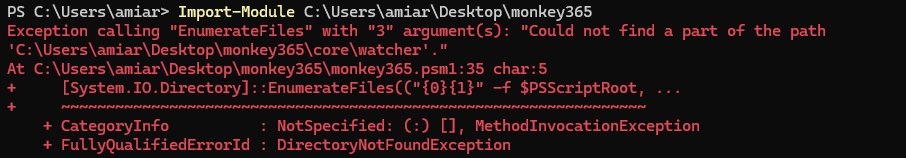
\includegraphics[scale=0.55]{images/ErreurImportationWatcher.png}}
        \caption{Erreur importation module}
    \end{center}
\end{figure}

Ensuite, lors de l'exécution des audits sur SharePoint, Teams et OneDrive, des erreurs de droits d'accès ont été rencontrées. Ces services dépendent de SharePoint pour certaines configurations, et les erreurs de droits ont empêché la collecte des données nécessaires pour les audits, compliquant ainsi l'évaluation des configurations. La prochaine image montre l'erreur de droits d'accès.

\begin{figure}[H]
    \begin{center}
        \fbox{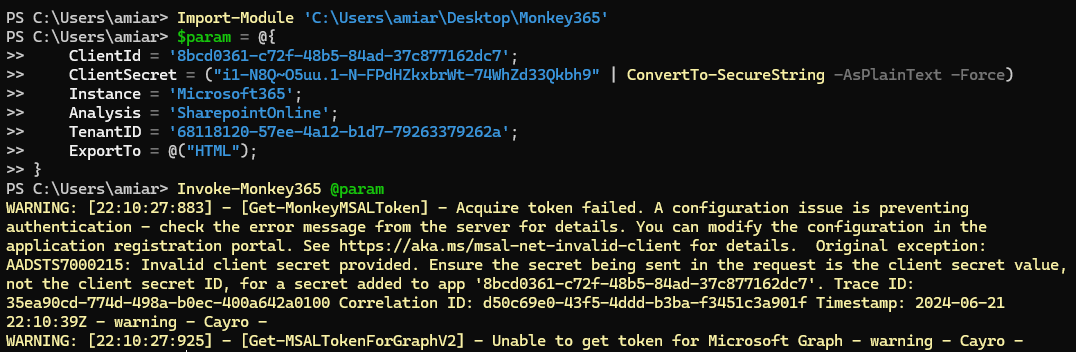
\includegraphics[scale=0.50]{images/ErreurDroits.png}}
        \caption{Erreur droits Sharepoint}
    \end{center}
\end{figure}

Enfin, lors de l'exécution de l'audit Azure, j'ai rencontré une erreur en raison de l'absence de souscription Azure dans notre environnement de test. Cette absence de souscription a empêché l'audit de récupérer les informations requises pour évaluer les configurations Azure. La prochaine image démontre cette erreur liée à l'absence de souscription.

\begin{figure}[H]
    \begin{center}
        \fbox{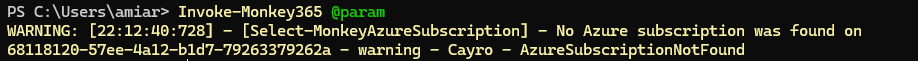
\includegraphics[scale=0.7]{images/ErreurSubscription.png}}
        \caption{Erreur souscription Azure}
    \end{center}
\end{figure}

Ces problèmes ont nécessité une attention particulière, ainsi que l'intervention des membres de mon équipe et de plusieurs experts. Dans la section suivante, je discuterai des solutions que nous avons mises en place pour surmonter ces obstacles et permettre la poursuite du projet.

\subsection{Solutions apportées}

Pour résoudre le problème lié au module "watcher", ma première solution a été de créer un dossier vide nommé "watcher" dans le chemin dédié. Bien que cela ait fonctionné, je savais que ce n'était pas la meilleure façon de traiter ce problème. J'ai ensuite supprimé ce dossier et cherché les fichiers ou lignes de code appelant le module, afin de modifier ces derniers pour enlever la dépendance en supprimant la ligne qui appelait "watcher". Cette approche a également fonctionné, mais elle n'était pas satisfaisante à long terme. \textbf{Mauslem Z.} m'a suggéré de consulter les issues sur GitHub, et effectivement, j'ai trouvé que quelqu'un avait déjà signalé ce problème. Une réponse de l'auteur de Monkey365 indiquait qu'il y avait effectivement un problème en cours de correction et qu'il fallait utiliser la branche "dev" au lieu de la branche "main" pour obtenir une version fonctionnelle. En utilisant la branche "dev", nous avons trouvé le module "watcher" complet, ce qui nous a semblé plus sécurisé. Quelques jours plus tard, le créateur de l'outil a publié une nouvelle version sans ce problème, que nous avons adoptée pour nos modifications.

Pour les problèmes de droits d'accès lors des audits \textbf{SharePoint}, \textbf{Teams} et \textbf{OneDrive}, je me suis référé à la documentation de \textbf{Monkey365}, qui explique qu'il existe trois méthodes d'authentification : directement avec mon compte, avec un \textbf{certificat}, et avec un \textbf{code secret}. Les deux dernières méthodes nécessitent que l'application soit enregistrée sur notre tenant. Pour des raisons de sécurité, j'ai d'abord évité d'utiliser mon compte directement. En utilisant mes connaissances sur \textbf{Azure} et les ressources en ligne telles que StackOverFlow, reddit et autres blogs, j'ai créé une application dans \textbf{Microsoft Entra ID} (le répertoire de tout le tenant), généré un code secret et configuré l'outil pour se connecter. Cependant, cette méthode nécessitait des droits d'accès spécifiques. En tant qu'administrateur, j'ai pu attribuer les droits nécessaires conformément à la documentation, mais j'ai tout de même rencontré des erreurs lors de l'exécution des audits. En essayant avec un certificat, j'ai rencontré le même problème. Après avoir relu la documentation, j'ai trouvé un tableau qui présente les types d'authentification et les services auxquels l'outil peut accéder. Ce tableau est présenté ci-dessous. J'ai découvert que l'authentification par code secret est très limitée, mais l'authentification par certificat devrait fonctionner. En discutant avec mon équipe, nous avons appris que Microsoft met à jour très fréquemment ses politiques de sécurité, ce qui pourrait expliquer les problèmes rencontrés. La seule solution qui restait était l'authentification directe avec mon compte, qui prend les droits "délégués". Pour cette solution, comme l'application va se voir déléguer des droits, il est nécessaire que le compte utilisé pour lancer un audit soit administrateur du service concerné. Par exemple, pour lancer un audit de SharePoint, le compte doit être administrateur SharePoint, et de même pour les autres services. Un administrateur global, en revanche, peut lancer des audits de tous les services ou de plusieurs services simultanément, ce qui est mon cas. En utilisant mon compte administrateur global, l'outil a fonctionné correctement. Cependant, nous devons rester vigilants car la source de l'outil n'est pas totalement fiable. Je discuterai des vérifications de sécurité dans la prochaine sous-partie.

\begin{figure}[H]
    \begin{center}
        \fbox{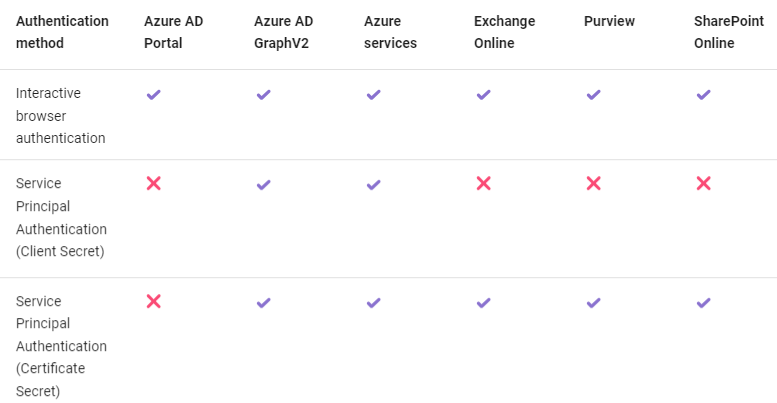
\includegraphics[scale=0.7]{images/tabledeservices.png}}
        \caption{Méthodes d'authentification prises en charge par service}
    \end{center}
\end{figure}

Pour le problème de souscription \textbf{Azure}, j'ai remonté le problème à mon équipe, et on m'a conseillé de ne pas trop me focaliser dessus pour l'instant, car la première version du projet ne nécessite pas l'analyse des services cloud donc pas d'abonnements \textbf{Azure}. On m'a recommandé de me concentrer sur notre objectif principal afin de progresser, car les problèmes précédents nous ont déjà coûté beaucoup de temps.

Ces solutions, bien que variées et parfois complexes, m'ont permis de surmonter les obstacles rencontrés et de faire avancer le projet de manière significative. Elles ont également permis d'utiliser la connaissance des experts et de favoriser la communication et la \textbf{coopération} au sein de l'équipe.

\subsection{Vérifications de sécurité}

En ce qui concerne la sécurité, nous avons effectué uniquement le minimum nécessaire pour nous assurer que l'utilisation de Monkey365 ne présente pas de risques majeurs. Pour ce faire, nous avons utilisé Fiddler pour vérifier les flux de données. Bien que Fiddler soit un nouvel outil pour moi, le concept ne m'était pas étranger, car j'avais déjà utilisé Wireshark à l'université.

Tout d'abord, j'ai lancé PowerShell et identifié l'ID du processus à suivre pour surveiller ses flux. J'ai ensuite configuré Fiddler pour écouter spécifiquement ce processus. En lançant un audit et en suivant tous les flux de données dans Fiddler, nous n'avons détecté aucun élément suspect, ce qui nous a quelque peu rassurés.

De plus, j'ai essayé d'examiner le code source de Monkey365. Bien que le code soit immense et difficile à analyser entièrement, une lecture partielle n'a révélé rien de suspect. Il est également important de noter que les audits ont été initialement exécutés dans des environnements de test et non sur des systèmes critiques ou officiels.

Après avoir été rassurés par ces vérifications, nous avons exécuté des audits sur d'autres tenants. Les résultats ont été positifs et l'outil a fonctionné correctement. Nous avons ainsi conclu ce Proof of Concept (POC) avec succès.

    

\section{Personnalisation de l'outil Monkey365}

\textit{Après avoir vérifié la sécurité de Monkey365 et validé son fonctionnement de base, nous avons entamé la phase de personnalisation de l'outil pour qu'il réponde spécifiquement à nos besoins. Cette personnalisation vise à transformer Monkey365 en une application adaptée à nos exigences particulières.}

\subsection{Adaptation du framework de sécurité}

Pour adapter Monkey365 à nos besoins spécifiques, j'ai d'abord cherché dans le code jusqu'à ce que je trouve le fichier contenant le framework de sécurité CIS. J'ai comparé ce fichier avec le véritable benchmark CIS, et il s'est avéré correct. Cependant, le framework était en format JSON, ce qui nécessitait des ajustements pour correspondre à notre situation spécifique. J'ai modifié certaines règles, en supprimé quelques-unes et ajusté d'autres.

Cette adaptation m'a donné l'idée de développer, à l'avenir, un générateur de JSON avec une interface où nous pourrions configurer les paramètres comme nous le souhaitons, ou importer une baseline déjà établie comme le CIS. Nous pourrions alors apporter des modifications ou conserver la configuration telle quelle et générer le JSON correspondant. Cette idée a été bien accueillie par l'équipe et a été prise en compte pour une utilisation future.

\subsection{Modification de l'interface utilisateur}

Pour commencer, j'ai supprimé toutes les références à "monkey" dans le code. Étant donné la taille du code, cela risquait de casser l'outil. Pour faciliter cette tâche, j'ai utilisé mes connaissances et des recherches en ligne pour créer un \textbf{script PowerShell} qui parcourt les fichiers et les lignes de code afin de remplacer toutes les occurrences de "monkey" par "\textbf{audit}". Le script a bien fonctionné, mais le code s'est tout de même cassé. Pourquoi ? Parce que le script ne respectait pas les majuscules. Par exemple, "\textbf{Monkey}" devait être transformé en "\textbf{Audit}" et non en "audit". Il y a eu de nombreux problèmes liés à cette subtilité.

Même si mon script fonctionnait bien, il ne s'adaptait pas parfaitement à la situation. J'ai cherché une solution alternative et trouvé que Visual Studio Code permettait de remplacer des mots en respectant les majuscules et minuscules. J'ai donc pu effectuer le changement de manière semi-manuelle. Après avoir vérifié que mon changement n'affectait pas le fonctionnement du code, j'étais satisfait. Désormais, pour lancer un audit, nous utilisons "\textbf{Invoke-Audit}" au lieu de "\textbf{Invoke-Monkey}".

Ensuite, je me suis attaqué au front-end et j'ai découvert quelque chose de très étrange : il n'y avait aucun fichier \textbf{HTML}, \textbf{CSS}, ni \textbf{JavaScript}, seulement du \textbf{PowerShell}. Comment alors le \textbf{HTML} est-il généré ? J'ai passé du temps à découvrir qu'une variable PowerShell cachée au fond du code contenait un template \textbf{HTML} en string, en une seule ligne, qui n'était qu'un appel aux styles, scripts et librairies. Mais l'énigme n'était pas encore résolue. En traçant un peu plus, j'ai trouvé un fichier zip nommé "assets" contenant tous les logos, librairies externes comme \textbf{Bootstrap}, \textbf{CSS} et \textbf{JS}. Ce qui m'a impressionné, c'est que tout était contenu dans un fichier zip. Le code générait le \textbf{HTML} à partir du template en extrayant le zip dans le dossier de sortie.

Avec cette découverte, j'ai pu faire les modifications nécessaires au niveau du \textbf{front-end}, en changeant les styles et scripts dans le fichier "assets.zip". J'ai continué à chercher jusqu'à trouver que chaque fois qu'une analyse d'audit se lançait, elle appelait des scripts PowerShell pour générer des éléments HTML, comme "New-SideBar.ps1" pour la barre de navigation ou "New-HtmlCard.ps1" pour les cartes HTML. Grâce à toutes ces découvertes, j'ai modifié du \textbf{PowerShell} et du \textbf{CSS} dans "assets.zip" pour donner de nouvelles couleurs à notre outil et changer le logo, afin de prouver ma capacité à effectuer des modifications au niveau du \textbf{front-end}.

Les deux images suivantes montrent l'édition officielle de Monkey365 et notre petite modification de personnalisation. Après avoir prouvé ces changements, nous avons sollicité notre coéquipier, \textbf{Pisda}, graphiste designer, pour créer un nouveau design pour notre outil. Nous avons donc temporairement arrêté les modifications \textbf{front-end} en attendant sa maquette.

\begin{figure}[H]
    \begin{center}
        \fbox{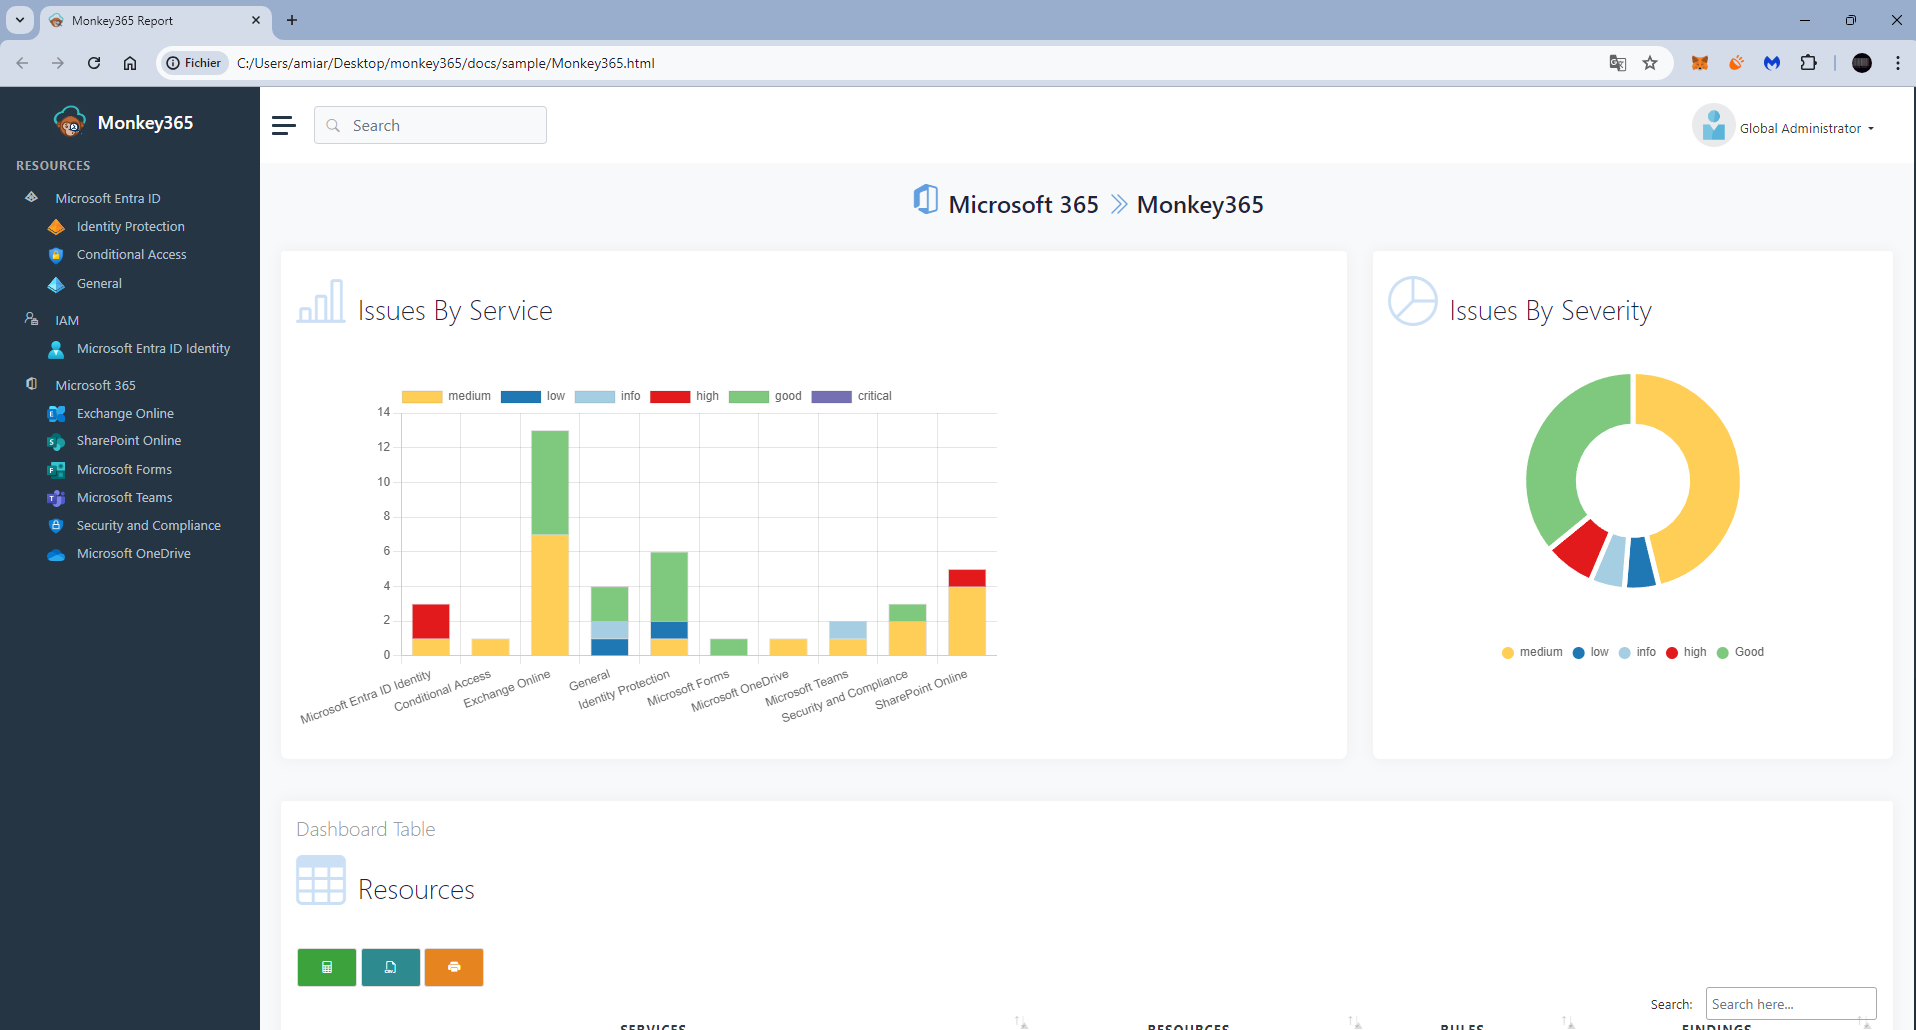
\includegraphics[scale=0.245]{images/Monkey365html.png}}
        \caption{Interface Monkey365 avant changement}
    \end{center}
\end{figure}

\begin{figure}[H]
    \begin{center}
        \fbox{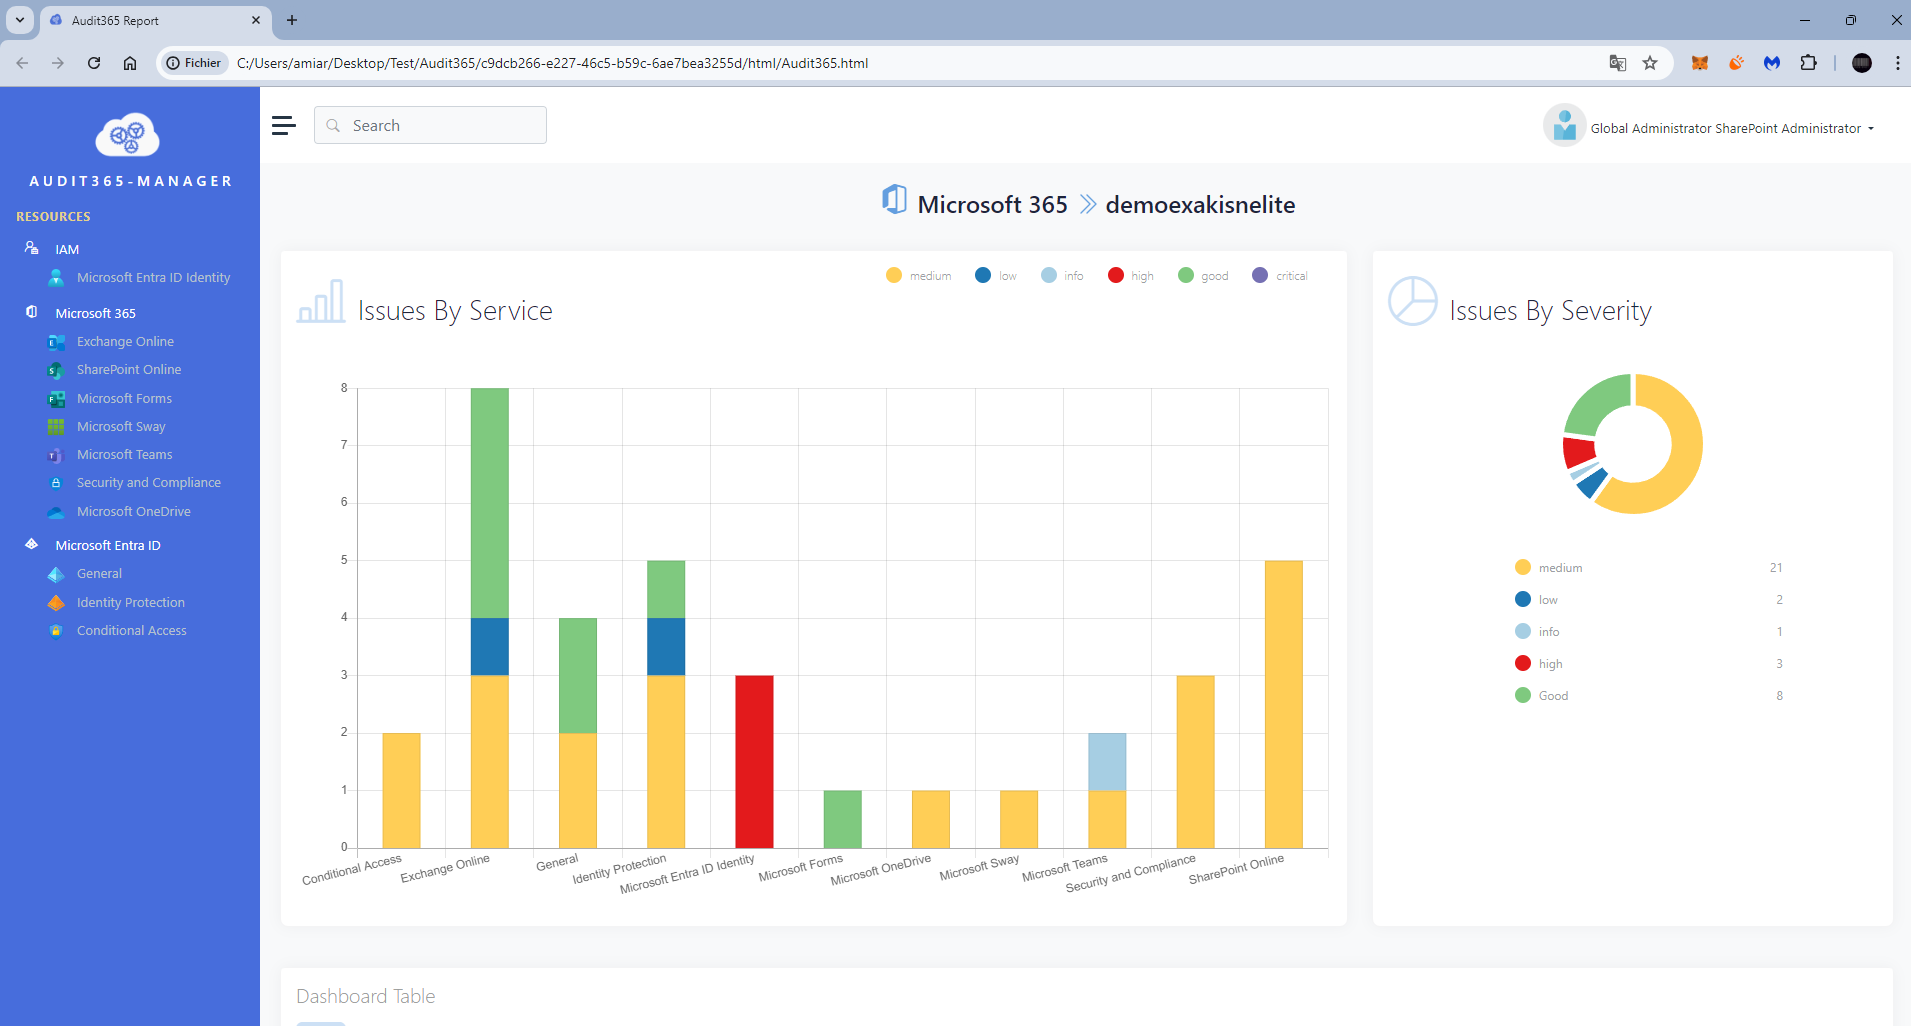
\includegraphics[scale=0.245]{images/audit365html.png}}
        \caption{Interface Monkey365 apres changement (Audit365)}
    \end{center}
\end{figure}

\subsection{Conception de l’architecture de l'application}

On m'a confié la tâche de concevoir une architecture pour notre application. Bien que cette mission dépasse largement mon niveau actuel, l'objectif était que je puisse apprendre de mes erreurs après validation par un expert. Voici la conception que j'ai réalisée.

L'architecture proposée repose sur plusieurs composants clés pour assurer une gestion efficace et sécurisée des audits :

\begin{itemize}
    \item \textbf{Utilisateurs et Entra ID} : Les utilisateurs s'authentifient via Entra ID, qui gère l'authentification et l'autorisation des accès.
    \item \textbf{Web App} : Cette application web, déployée via un App Service Plan, est le cœur du système. Elle héberge le backend (Rest API), le frontend (interface utilisateur), ainsi qu'un conteneur de l'application.
    \item \textbf{Function Apps} : Ces applications de fonctions, qui sont des services serverless, exécutent les scripts PowerShell nécessaires à l'importation des modules et à l'invocation des audits.
    \item \textbf{Container Image} : Une image de conteneur est utilisée pour déployer l'outil Monkey365 et les composants nécessaires de manière cohérente et reproductible.
    \item \textbf{Monkey365} : Cet outil interroge les environnements Azure et Microsoft 365 pour réaliser les audits.
    \item \textbf{Azure SQL Database} : La base de données stocke les résultats des audits et autres données nécessaires au fonctionnement de l'application.
    \item \textbf{Outputs} : Les résultats des audits sont initialement diffusés en page HTML, mais peuvent être transformés en divers formats, y compris Excel, JSON, CSV et CLIXML.
    \item \textbf{Diagnostic logs and metric data} : Les données de diagnostic et les métriques sont envoyées à Log Analytics et Azure Monitor pour surveiller la santé de l'application.
\end{itemize}

L'image suivante montre l'architecture conçue par moi sur l'application Lucidchart :

\begin{figure}[H]
    \centering
    \fbox{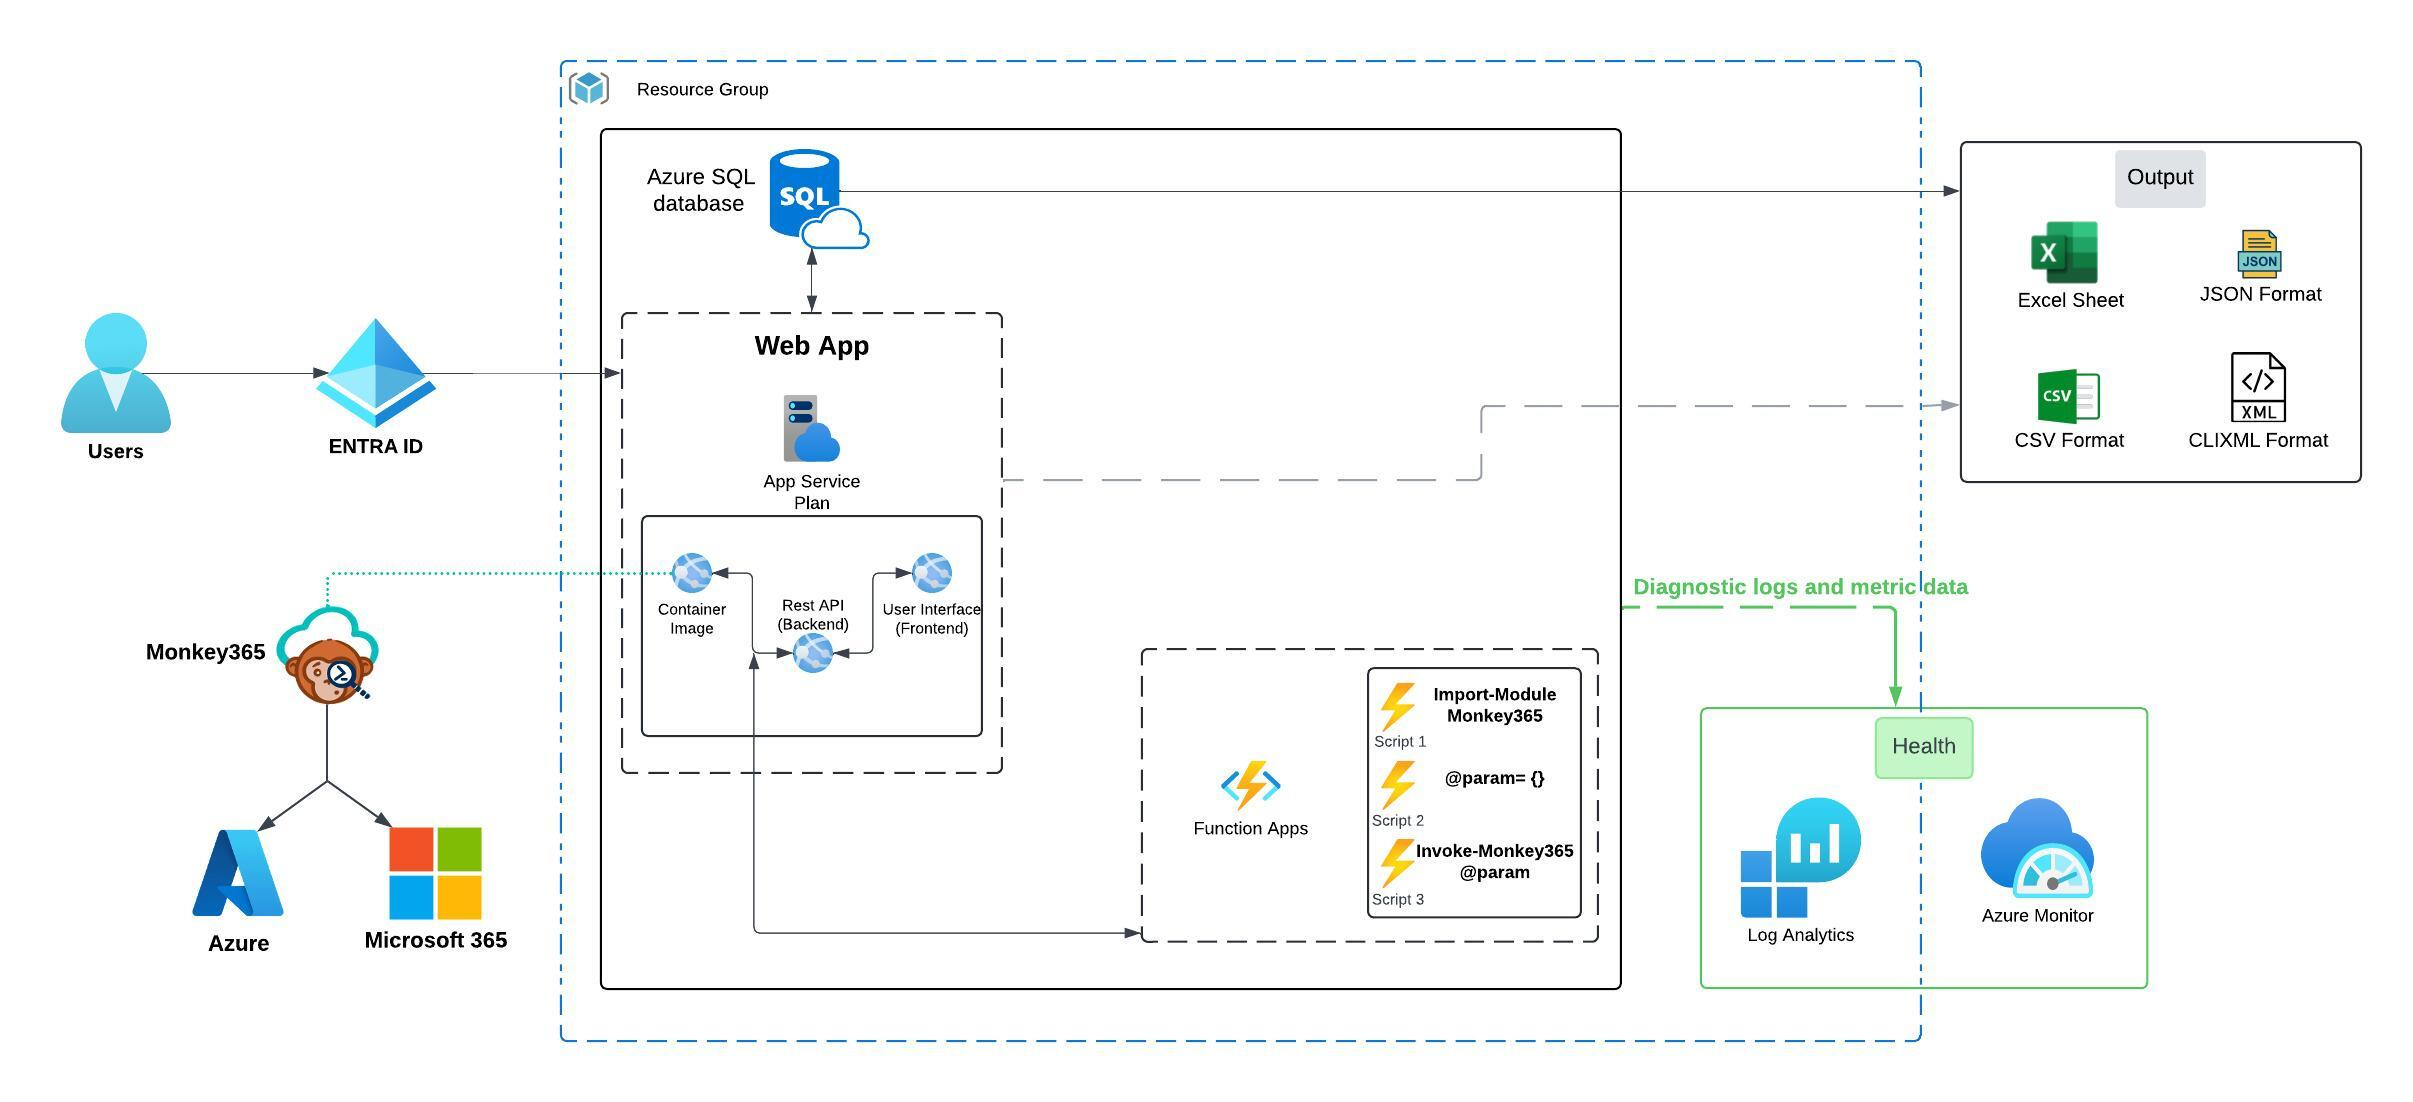
\includegraphics[scale=0.5]{images/ArchitectureAudit.jpeg}}
    \caption{Architecture de déploiement proposée pour l'application}
\end{figure}

Cette architecture permet une intégration fluide entre les différents composants et assure que les audits peuvent être exécutés efficacement et en toute sécurité. L'architecture a été partiellement validée par l'équipe, mais nécessite toujours l'approbation finale d'un architecte cloud, que nous attendons pour valider totalement ou apporter de petites modifications.

\section{Gestion du dépôt du projet}

Pour faciliter la gestion du code source et assurer une collaboration efficace, nous avons décidé d'utiliser un dépôt Git pour notre projet. Actuellement, le code du projet \textbf{Audit365 Manager} est hébergé sur mon dépôt personnel GitHub en visibilité privée. Cette solution temporaire nous permet de suivre les modifications et de travailler de manière collaborative.

Cependant, pour une gestion plus sécurisée et professionnelle, nous prévoyons de migrer le projet vers un dépôt professionnel d'entreprise. Cette migration nécessitera l'intervention d'un expert en infrastructure et DevOps, que nous attendons pour configurer et sécuriser le dépôt d'entreprise. Ce dépôt centralisé permettra de mieux gérer les versions, de suivre les modifications apportées par chaque membre de l'équipe, et d'assurer une meilleure intégration continue et déploiement continu (CI/CD).

\section{Récapitulatif}

Ce chapitre a été consacré au \textbf{cadrage technique} du projet \textbf{Audit365 Manager}. Nous avons d'abord effectué une \textbf{analyse de l'existant}, en examinant le code de la librairie tierce Monkey365, et en développant et testant un \textbf{Proof of Concept (POC)}. Cette analyse nous a permis de vérifier que Monkey365 répondait à nos besoins, mais a également révélé plusieurs problèmes.

Ensuite, nous avons discuté des solutions apportées pour surmonter ces obstacles. Nous avons également effectué des \textbf{vérifications de sécurité} en utilisant Fiddler pour s'assurer qu'aucun flux de données suspect n'était présent.

La deuxième partie du chapitre a porté sur la \textbf{personnalisation de l'outil Monkey365}. Nous avons adapté le framework de sécurité pour l'aligner avec nos besoins spécifiques. J'ai également entrepris des modifications de l'interface utilisateur. Ces modifications ont été validées par l'équipe, mais un travail de design supplémentaire a été confié à notre graphiste.

Puis, j'ai conçu une \textbf{architecture de déploiement} pour notre application, décrivant comment les différents composants s'intègrent pour assurer une gestion efficace des audits. Cette architecture a été partiellement validée par l'équipe, mais nécessite toujours l'approbation finale d'un architecte cloud.

Enfin, nous avons discuté de la gestion du dépôt du projet, qui est actuellement hébergé sur mon dépôt personnel GitHub, en attendant la mise en place d'un dépôt d'entreprise pour une gestion plus professionnelle et sécurisée.

Ce chapitre marque la fin de la progression de mon travail à la date de rédaction de ce rapport. Cependant, le projet \textbf{Audit365 Manager} continue d'évoluer, et mon stage n'est pas encore terminé. Le prochain chapitre abordera les formations et les apprentissages dont j'ai pu bénéficier au cours de ce stage.
